\documentclass[12pt]{article}
\usepackage{preamble}
\usetikzlibrary{decorations.pathreplacing}
% -- document title --
\title{Impacts of Childcare Service on Mothers' Labor Supply: \\ 
       Evidence from Optional Separate Surnames in Japan\thanks{
        This proposal is not prepared for the thesis, but I am planning to use it if the optional separate surnames policy is implemented in Japan.
       }
       }
\author{Sakito Tango\thanks{id: 29246024, 
        email: \href{mailto:tango-sakito@g.ecc.u-tokyo.ac.jp}{tango-sakito@g.ecc.u-tokyo.ac.jp}
}
}
\date{\today}
% --------------------------

\begin{document}

\maketitle

\section{Research Question}
This proposal aims to answer the following questions: Do mothers work more if coetaneous children decrease and the childcare service becomes easier to access?   
I suggest the way of analyzing these questions with regression discontinuity design (RDD) using Japanese data. 
I use the introduction of optional separate surnames as an instrument, supposing that the policy is implemented in Japan.


\section{Motivation}
The relationship between fertility and mothers' labor supply is one of the most major topics in Japan. 
According to the Japanese National Fertility Survey in 2021 by National Institute of Population and Social Security Research, about 41\% of full-time working mothers stop working full-time after the birth of their first child.
It is important to provide the environment where mothers can work while raising children, in terms of promoting full-use of labor resources, female social advancement, and fertility rate.


In this context, the effectiveness of childcare service is a key issue. 
The expansion of childcare service is expected to reduce the burden of child-rearing on mothers and increase their labor supply, and the supply of it has been increasing according to Children and Families Agency. 
However, it requires a large budget to increase its supply, so it is integral to evaluate the effectiveness.


There exist a wide range of studies which estimate the effect of childcare service on mothers' labor supply.
\cite{Baker2008-vt} is one of the most famous studies which uses the introduction of childcare service in Quebec, Canada, and shows that the policy increased mothers' labor supply.
However, the evaluation of childcare service is still difficult due to the endogeneity problem. 
It is the government that decides the supply of childcare service, and the decision is likely to be correlated with the unobservable factors. 
Also, the government which increases the supply of childcare service is likely to implement other policies which promote mothers' labor supply.
If we ignore these endogeneity, the estimated effect of childcare service could be overestimated.


This paper suggests using the introduction of optional separate surnames as an instrument to deal with the endogeneity problem and estimate the effect of childcare service on mothers' labor supply and fertility.
Today, Japan does not allow married couples to have separate surnames.
However, the discussion on the introduction of optional separate surnames is spreading.
A survey by NHK in April 2024 reveals that 62\% of Japanese people support the introduction of optional separate surnames while 27\% oppose it (\cite{nhk}).
Although the political process of the introduction of optional separate surnames is still uncertain, the probability of the introduction in the coming years is not low given the current public opinion.


Suppose, in Japan, the introduction is decided and announced, but the implementation is scheduled for the next year.
Then, couples who want to have separate surnames may postpone their marriage until the implementation. 
It is plausible because it is very costly to marry before the implementation, share the same surname, and change it after the implementation, compared to marrying after the implementation.
Also, if marriage is postponed, the birth of children is likely to be postponed.
Therefore, the number of pregnancies could decline between the announcement and the implementation.
As a result, children whose parents get pregnant just before the announcement are expected to have fewer coetaneous children.


This reduction of coetaneous children leads to exogenous decline of demand for childcare service.
Hence, mothers who have children just before the announcement have better access to childcare service due to the exogenous slack of demand.
Using this exogenous variation, we can estimate the effect of childcare service on mothers' labor supply. 


Of course, there is no study which uses the introduction of optional separate surnames in Japan as an instrument.
This proposal potentially has a significant contribution to the literature.
Therefore, it is valuable to design the empirical strategy in advance and prepare for the implementation.


\section{Potential Institutional Background}
In this proposal, I assume that the optional separate surnames policy is implemented as follows: 
\begin{itemize}
  \item The policy is announced at some point. 
  \item A year later, the policy is implemented.
  \item All couples can choose whether to have separate surnames or not after the implementation.
\end{itemize}
The important point is that there exists a lag between the announcement and the implementation.
Due to this lag, some couples who want to have separate surnames may postpone their marriage until the implementation, which could delay the birth of their children.
It is plausible to expect that there exists a lag because allowing separate surnames requires a wide range of administrative changes.
In this proposal, I assume the lag to be twelve months, but the actual lag could be longer or shorter if it exists.

\section{Empirical Model}
\subsection*{Explanation on Sample}
Figure \ref{fig:timeline} shows the timeline of the policy announcement and implementation.

\begin{figure}[htbp]
\scalebox{0.8}{
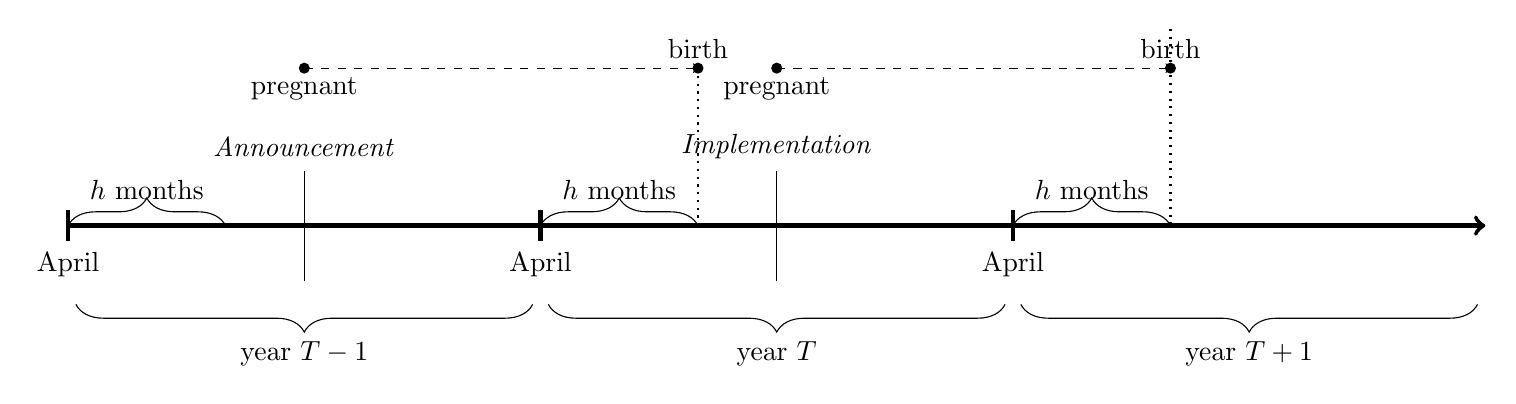
\begin{tikzpicture}

  % Draw the main timeline
  \draw[->,ultra thick] (0,0) -- (18,0);
  % \draw[->] (0,3) -- (18,3);
  
  % Annotations on the top line
  \node at (3, 3.5-2-0.5) {\textit{Announcement}};
  \node at (9, 3.5-2-0.5) {\textit{Implementation}};
  % \draw (3,3.2) -- (3,2.8);
  % \draw (9,3.2) -- (9,2.8);
  \draw (3,3.2-2-0.5) -- (3,2.8-3-0.5);
  \draw (9,3.2-2-0.5) -- (9,2.8-3-0.5);
  
  % Pregnant and birth labels on the top line
  \node[below] at (3, 2.5-0.5) {pregnant};
  \node[above] at (8, 2.5-0.5) {birth};
  \node[below] at (9, 2.5-0.5) {pregnant};
  \node[above] at (14, 2.5-0.5) {birth};
  \fill (3, 2.5-0.5) circle (2pt);
  \fill (8, 2.5-0.5) circle (2pt);
  \fill (9, 2.5-0.5) circle (2pt);
  \fill (14, 2.5-0.5) circle (2pt);
  \draw[->,dashed] (3, 2.5-0.5) -- (8, 2.5-0.5);
  \draw[->,dashed] (9, 2.5-0.5) -- (14, 2.5-0.5);
  \draw[dotted,thick] (8, 2.5-0.5) -- (8, 0);
  \draw[dotted,thick] (14, 2.5) -- (14, 0);

  \draw[decorate, decoration={brace, amplitude=10pt}] (0,0) -- (2,0) node[midway, above,yshift=6pt] {$h$ months};
  \draw[decorate, decoration={brace, amplitude=10pt}] (6,0) -- (8,0) node[midway, above,yshift=6pt] {$h$ months};
  \draw[decorate, decoration={brace, amplitude=10pt}] (12,0) -- (14,0) node[midway, above,yshift=6pt] {$h$ months};
  
  % Lower timeline labels
  \node at (0, -0.5) {April};
  \node at (6, -0.5) {April};
  \node at (12, -0.5) {April};
  \draw[ultra thick] (0, 0.2) -- (0, -0.2);
  \draw[ultra thick] (6, 0.2) -- (6, -0.2);
  \draw[ultra thick] (12, 0.2) -- (12, -0.2);
  
  % Labels for cohort periods
  \draw[decorate, decoration={brace, amplitude=10pt, mirror}] (0.1,-1) -- (5.9,-1) node[midway, below,yshift=-10pt] {year $T-1$};
  \draw[decorate, decoration={brace, amplitude=10pt, mirror}] (6.1,-1) -- (11.9,-1) node[midway, below,yshift=-10pt] {year $T$};
  \draw[decorate, decoration={brace, amplitude=10pt, mirror}] (12.1,-1) -- (17.9,-1) node[midway, below,yshift=-10pt] {year $T+1$};
  
  \end{tikzpicture}
}
  \caption{Timeline}
  \label{fig:timeline}
\end{figure}

For simplicity, dismiss the variation in the durations of pregnancy across mothers. 
Also, suppose there is a year of lag between the announcement and the implementation.


I denote a fiscal year as year $T$ if a mother who gets pregnant her first child just before the announcement gives birth in that fiscal year.
I also denote a year before year $T$ as year $T-1$, and a year after year $T$ as year $T+1$, and so on.
In the same way, I divide mothers and their first children into groups depending on the birth date of their first child. 
I denote the group of mothers whose first child is born in year $T$ as group $T$, and so on.
This classification holds in general, independent of the timing of the announcement.


See the characteristic of each group.
All mothers in group $T-1$ are pregnant before the announcement, which means they are not affected by the announcement.
In group $T$, some mothers whose first child is born in first $h$ months in year $T$ are pregnant before the announcement, and the others are pregnant after the announcement.
Denote the former as subgroup $h$ and the latter as subgroup $h^c$.
As I explained above, due to the postponement of marriage and pregnancy, the number of children in subgroup $h^c$ is expected to be smaller than that in subgroup $h$ in group $T$.


It is plausible to expect that the subgroup $h$ of group $T$ and the subgroup $h$ of group $T-1$ have the \textit{ex-ante} identical characteristics.
Both do not know the policy when deciding pregnancy, and their children's birthdays are within the first $h$ months of each year. 
The only difference is the number of coetaneous children.
The subgroup $h^c$ of group $T$ is pregnant after announcement but before implementation, so the number of children is expected to be smaller than that in subgroup $h^c$ of group $T-1$.


\subsection*{Regression Formulation}
Formulate the regression.
I restrict the sample to mothers in subgroup $h$ of group $T$ and subgroup $h$ of group $T-1$.


Denote $X_{i,s}$ as the dummy variable which takes 1 if mother $i$ can access childcare service when her child is $s$ years old, and 0 otherwise.
The causal relationship of interest is as follows:
\begin{align}
  Y_{i,s} = \alpha + \beta X_{i,s} + \vb{W}_{i}'\vb{\gamma} + \epsilon_{i,s}, \label{naive}
\end{align}
where $Y_{i,s}$ is the outcome which measures the labor supply of mother $i$ when her child is $s$ years old.
For example, $Y_{i,s}$ could be the working hours. 
$\vb{W}_{i}$ is the vector of control variables which includes the predetermined characteristics of mother $i$, such as age of marriage, education, income of husband, and so on.


Of course, the endogeneity problem exists. 
Mothers who want to work more are likely to be more enthusiastic about applying for childcare service, so na\"ive estimation of $\beta$ could be overestimated.
To deal with the endogeneity, use fuzzy RDD.
I use the birth date of the first child as the running variable, and the cutoff point is April of year $T$.
\todo{check}
At this point, the number of coetaneous children discontinuously decreases, and thus the access to childcare service discontinuously becomes easier.
I refer to \cite{Dahl2014-bm} for the specification and estimate by 2SLS.


I formulate a first step regression as following: 
\begin{align}
  X_{i,s} = \varphi + \vb{1}[t_b\geq c](g_l(t_b-c)+\lambda) + \vb{1}[t_b<c](g_r((t_b-c))) + \vb{W}_{i}'\vb{\gamma} + \varsigma_{i,s}, \label{step1} 
\end{align}
where $\vb{1}$ is the indicator function. 
$t_b$ is the date of birth of the first child and $c$ is the cutoff point, April of year $T$. 
Therefore, the indicator function takes 1 if the birth date is after April of year $T$, which means the mother is in subgroup $h$ of group $T$.
$g_l$ and $g_r$ are the unknown polynomial functions.
Note that the sample is restricted to mothers in subgroup $h$ of group $T$ and subgroup $h$ of group $T-1$.


After estimating \eqref{step1}, I estimate the second step regression as following:
\begin{align}
  Y_{i,s} = \alpha + \beta \hat{X}_{i,s} + \vb{1}[t_b\geq c](g_l(t_b-c)) + \vb{1}[t_b<c](g_r((t_b-c))) + \vb{W}_{i}'\vb{\gamma} + \epsilon_{i,s}. \label{step2}
\end{align}
Then, the resulted $\hat{\beta}$ is the estimation of the causal effect of interest. 
It represents the effect of easier access to childcare service on mothers' labor supply when their child is $s$ years old.


\subsection*{Validation of RDD}
In this subsection, I validate this identification strategy with RDD. 


First, the existence of the discontinuity is plausible.
If the introduction of optional separate surnames is announced, couples who want separate surnames are likely to postpone their marriage until the implementation.
This is because it requires to change surname twice, if they marry before the implementation, share the same surname, and change it after the implementation. 
This is very costly and inconvenient, while postponing marriage less than a year is less costly.
Also, the fraction of newly married couples who want separate surnames is expected to be significant at the time of the announcement, considering the public opinion.
Therefore, it is plausible that the number of children discontinuously decreases at the cutoff point, and thus the access to the childcare service, $X_{i,s}$, discontinuously becomes easier.


Second, the running variable, the birth date of the first child, satisfies the three conditions: (i) positive density at the cutoff, (ii) continuous impact of the running variable at the cutoff, and (iii) incomplete control of the running variable.
(i) is satisfied because the birth date is uniformly distributed across the year. 
(ii) is satisfied because 
  

\section{Data}



\nocite{*}
\bibliography{research_proposal}
\bibliographystyle{econ}

\end{document}